\fancyhead[R]{Berkay Günes}

In this section, we elucidate our methodology and approaches concerning the various machine learning models 
that we have developed for the Bomberman game agent. We will also substantiate what has proven effective, articulate 
the concepts we have discarded, and expound upon the rationale for ultimately selecting the model we have submitted.

\subsection{Q-learning}

Reinforcement learning (RL) is a subfield of machine learning that focuses on training agents to make a decision given a state representation of the world through trial and error, aiming to maximize a cumulative reward. Q-learning is a fundamental RL algorithm that has played a pivotal role in solving various problems in robotics, gaming, and more. In this section, we will introduce Q-learning and then focus on Deep Q-Networks (DQNs), explaining how they differ from traditional Q-tables.

\subsubsection{Q-Learning}

Q-learning is a model-free reinforcement learning algorithm that learns an action-value function, denoted as \(Q(s, a)\), where 's' represents the state, and 'a' represents the action. The Q-value of a state-action pair quantifies the expected cumulative reward an agent can achieve starting from that state and taking a specific action. The primary goal of Q-learning is to find the optimal policy, which is a mapping of states to actions that maximizes the expected cumulative reward over time.

The Q-learning algorithm updates Q-values iteratively through the following equation:

\begin{equation}
	Q(s_t, a_t) \leftarrow Q(s_t, a_t) + \alpha \left[ r_t + \gamma \max_a Q(s_{t+1}, a) - Q(s_t, a_t) \right]
\end{equation}

Here, \(s_t\) represents the current state, \(a_t\) is the chosen action, \(r_t\) is the immediate reward received, \(\gamma\) is the discount factor, and \(\alpha\) is the learning rate.

Q-learning operates in discrete state and action spaces, making it highly suitable for problems where these spaces are well-defined, such as board games and simple robotic tasks. However, Q-learning faces limitations when dealing big feature spaces as the Q-tables grow exponentially, which led to the development of Deep Q-Networks (DQNs).

\subsubsection{Deep Q-Networks}

Deep Q-Networks (DQNs) are a class of neural network-based reinforcement learning algorithms that combine deep learning with Q-learning principles. They address the limitations of Q-learning by approximating the Q-value function using a neural network instead of a Q-table. This enables DQNs to handle complex and continuous state spaces, making them highly effective in tasks like image-based game playing and autonomous driving.

Key differences between DQNs and traditional Q-tables include:

\begin{enumerate}
	\item \textbf{Function Approximation}: DQNs use a neural network to approximate the Q-values, allowing them to generalize across similar states. Traditional Q-learning relies on a discrete Q-table, which is not practical for large state spaces.
	
	\item \textbf{Experience Replay}: DQNs store experiences (state, action, reward, next state) in a replay buffer and sample mini-batches during training. This stabilizes learning by breaking the temporal correlation between experiences and mitigating the risk of convergence to suboptimal policies.
	
	\item \textbf{Target Network}: To stabilize training, DQNs use two networks: the target network and the policy network. The target network lags behind the policy network, and its Q-values are used as targets for training. This helps in reducing the variance of Q-value estimates during training.
\end{enumerate}

% ----------------------------------------------------------------------------------------------------------------------------------------------

\subsection{Neural Networks}
Neural networks, often referred to as artificial neural networks (ANNs), are a class of machine learning models inspired by the structure and function of the human brain. They have gained significant popularity in recent years due to their remarkable ability to learn and generalize from data, making them versatile tools for a wide range of tasks, from image recognition to natural language processing. While they have been around for a rather long time, it was only in the recent decade that computational power became sufficient to train networks that are large enough to be useful. Also, the amount of available data for training has dramatically increased over the years.

\subsubsection{Basic Structure of a Neural Network}

At its core, a neural network is composed of interconnected nodes, known as neurons or artificial neurons, organized into layers. The three primary types of layers in a neural network are:

\begin{enumerate}
	\item \textbf{Input Layer}: This layer consists of neurons that receive the initial data or features. Each neuron corresponds to a specific feature, and its value represents the magnitude of that feature.
	
	\item \textbf{Hidden Layers}: Hidden layers are intermediary layers between the input and output layers. They process the input data through a series of weighted connections and nonlinear activation functions.
	
	\item \textbf{Output Layer}: The output layer produces the final results or predictions of the neural network's task. The number of neurons in this layer depends on the problem, with each neuron typically corresponding to a different class or a particular aspect of the prediction.
\end{enumerate}

\subsubsection{Working Principle of Neurons}

Each neuron in a neural network performs a simple but crucial task. It takes in a weighted sum of its inputs, adds a bias term, and passes this value through an activation function to produce an output, thus each neuron in the network has a number of free parameters that need to be determined by training. The equation for the operation of a neuron is be defined as:

\begin{equation}
	\text{Output} = \text{Activation}\left(\sum_{i=1}^{n} (\text{Input}_i \times \text{Weight}_i) + \text{Bias}\right)
\end{equation}

\subsubsection{Training a Neural Network}

The essence of neural networks lies in their ability to approximate any function, and thus "learn" a relation between input and output data, no matter how complex this relationship might be. This learning process involves adjusting the weights and biases of the neurons to minimize a specific loss or error function. Here's an overview of the training process:

\begin{enumerate}
	\item \textbf{Forward Pass}: During the forward pass, input data is propagated through the network layer by layer. Neurons compute their outputs using the weighted sum and activation function.
	
	\item \textbf{Loss Calculation}: The output of the neural network is compared to the ground truth or target values, and a loss (error) is calculated. The choice of loss function depends on the task. A few different examples are given in \ref{loss}.
	
	\item \textbf{Backpropagation}: In the backpropagation step, the gradient of the loss with respect to the network's parameters (weights and biases) is computed using the chain rule. This gradient indicates how much each parameter should be adjusted to minimize the loss.
	
	\item \textbf{Optimization}: The gradients are used to update the network's parameters in the opposite direction of the gradient. This process is repeated iteratively until the loss converges to a minimum.
\end{enumerate}

\subsubsection{Batch Normalization}

Batch Normalization is a widely used technique in deep learning, specifically designed to address training instability and accelerate convergence in neural networks. It operates by normalizing the activations of each layer within mini-batches during training and introduce learnable parameters (scale and shift) to allow the network to adapt and fine-tune the normalized activations.
These are then passed through the activation function and used in subsequent layers for forward and backward passes.
\\ \\
\textbf{Advantages of Batch Normalization:} \\
Batch Normalization helps mitigate issues like vanishing and exploding gradients, making it easier to train deep networks. By normalizing the activations, it maintains a more consistent and stable gradient flow during backpropagation.
Neural networks with Batch Normalization also tend to converge faster. The normalization of activations helps prevent the network from getting stuck in plateaus, enabling quicker convergence to a better solution.
Batch Normalization introduces a degree of regularization by reducing internal covariate shift (the change in the distribution of activations between layers). This often leads to better generalization and reduced overfitting.


% ----------------------------------------------------------------------------------------------------------------------------------------------
\newpage
\subsection{Optimizer}

In machine learning, optimization plays a vital role in training deep neural networks. Optimizers are algorithms responsible for adjusting the model's parameters to minimize a loss function during training. They control how the model learns and, consequently, impact its convergence speed and overall performance. Two popular optimizers used in deep learning are RMSprop and AdamW. In this section, we will explain the role of optimizers and delve into the mechanisms of RMSprop and AdamW.

Optimizers in machine learning are responsible for updating the weights and biases of a neural network to minimize a chosen loss function. The primary goal is to find the optimal set of parameters that result in the lowest possible loss. This is achieved through an iterative process that involves computing gradients of the loss with respect to the model's parameters and adjusting these parameters in the direction that reduces the loss.

\subsubsection{RMSprop}

RMSprop (Root Mean Square Propagation) is an adaptive learning rate optimizer designed to address the issue of slow convergence in stochastic gradient descent (SGD) and is defined by:


\begin{align}
	v_t &= \beta \cdot v_{t-1} + (1 - \beta) \cdot (\nabla J(\theta_t))^2 
	\\
	\theta_{t+1} &= \theta_t - \frac{\alpha}{\sqrt{v_t + \epsilon}} \cdot \nabla J(\theta_t)
\end{align}    

Where \(v_t\) describes the moving average of squared gradients, \(\beta\) the decay rate for the moving average (usually set to a value like 0.9), \(\nabla J(\theta_t)\) represents the gradient of the loss with respect to the model parameters \(\theta_t\), \(\alpha\) is the learning rate and\(\epsilon\) is a small constant (typically used to avoid division by zero).

RMSprop works by maintaing a moving average of squared gradients for each parameter. It then adapts the learning rates individually for each parameter by dividing the current gradient by the square root of the moving average of squared gradients.
This adaptation helps to scale down the learning rate for parameters with high variance in gradients and scale up the learning rate for those with low variance.
RMSprop includes a smoothing term to avoid dividing by very small values, ensuring stable convergence.

RMSprop is well-suited for tasks with non-stationary objectives or sparse data. It helps mitigate the vanishing and exploding gradient problems and often converges faster than traditional SGD.

\subsubsection{AdamW}

AdamW (Adam with Weight Decay) is a variant of the Adam optimizer that addresses weight decay issues. AdamW incorporates L2 regularization (weight decay) directly into the parameter update step, unlike the original Adam optimizer, which applies weight decay as an additional term after the parameter update. It is defined by:

\begin{align}
	m_t &= \beta_1 \cdot m_{t-1} + (1 - \beta_1) \cdot \nabla J(\theta_t) \\
	v_t &= \beta_2 \cdot v_{t-1} + (1 - \beta_2) \cdot (\nabla J(\theta_t))^2 \\
	\hat{m}_t &= \frac{m_t}{1 - \beta_1^t} \\
	\hat{v}_t &= \frac{v_t}{1 - \beta_2^t} \\
	\theta_{t+1} &= \theta_t - \frac{\alpha}{\sqrt{\hat{v}_t + \epsilon}} \cdot \hat{m}_t - \lambda \cdot \theta_t
\end{align}

Where \(m_t\) and \(v_t\) are the first and second moments of gradients, respectively, \(\beta_1\) and \(\beta_2\) are the exponential decay rates for the first and second moments (typically set to values like 0.9 and 0.999), \(\hat{m}_t\) and \(\hat{v}_t\) are bias-corrected estimates of the moments, \(\nabla J(\theta_t)\) represents the gradient of the loss with respect to the model parameters \(\theta_t\), \(\alpha\) is the learning rate, \(\epsilon\) is a small constant and \(\lambda\) is the weight decay term, which adds L2 regularization to the parameter updates. \\
AdamW computes the gradients of the loss and updates the moving averages of the first and second moments of gradients.
It then includes an L2 regularization term in the parameter update step, which helps prevent overfitting.
By integrating weight decay, AdamW offers better generalization and improved performance in tasks with large neural networks.\\

AdamW is generally well-suited for a wide range of deep learning tasks and is particularly effective when dealing with large networks and complex datasets.

\subsubsection{Choosing the Right Optimizer}

The choice between RMSprop and AdamW depends on the specific characteristics of the deep learning task:

\begin{itemize}
	\item \textbf{RMSprop}: When dealing with non-stationary objectives, sparse data, or tasks where adaptive learning rates are crucial. It can help in scenarios where the learning rate needs to vary across parameters.
	
	\item \textbf{AdamW}: When you require effective regularization through weight decay, especially in large neural networks with many parameters. It is suitable for tasks where preventing overfitting is a top priority.
\end{itemize}

In practice, experimenting with both optimizers on the specific dataset and model architecture is often the best way to determine which one performs better for the task.

% ----------------------------------------------------------------------------------------------------------------------------------------------
\newpage
\subsection{Loss Functions} \label{loss}

Loss functions play a crucial role in training neural networks. They quantify the difference between the predicted outputs of the model and the ground truth labels. Different loss functions are used for different types of tasks and data.

\subsubsection{Cross-Entropy Loss} \label{sec:crossentropy}

Cross-entropy loss, often used in classification tasks, measures the dissimilarity between predicted class probabilities and the true class labels. It is particularly suitable for problems where the outputs are probability distributions.

The equation for binary cross-entropy loss for a single example is:

\begin{align}
	\text{Binary Cross-Entropy Loss} = -\left(y \log(\hat{y}) + (1 - y) \log(1 - \hat{y})\right)
\end{align}

Preferred Use Case: Cross-entropy loss is commonly used in classification tasks, including image classification and natural language processing.

\subsubsection{Huber Loss}

Huber loss is a robust loss function that combines the best properties of Mean Absolute Error (MAE) and Mean Squared Error (MSE) loss functions. It is less sensitive to outliers and provides a smoother gradient compared to MSE.

The Huber loss is defined as:

\begin{align}
	\text{Huber Loss} = \begin{cases}
		\frac{1}{2}(\hat{y} - y)^2, & \text{if } |\hat{y} - y| \leq \delta \\
		\delta|\hat{y} - y| - \frac{1}{2}\delta^2, & \text{otherwise}
	\end{cases}
\end{align}

Preferred Use Case: Huber loss is useful when dealing with regression problems where the dataset may contain outliers.

\subsubsection{Mean Squared Error (MSE) Loss}

Mean Squared Error (MSE) loss is a common loss function used for regression tasks. It measures the average squared difference between predicted and true values.

The equation for MSE loss is:

\begin{align}
	\text{MSE Loss} = \frac{1}{n} \sum_{i=1}^{n} (\hat{y}_i - y_i)^2    
\end{align}

Preferred Use Case: MSE loss is suitable for regression problems where the goal is to minimize the squared difference between predicted and true values.

\subsubsection{Smooth L1 Loss}

Smooth L1 loss is another loss function for regression that combines the best of both MAE and MSE. It is less sensitive to outliers than MSE and provides a smooth gradient.

The equation for Smooth L1 loss is:

\begin{align}
	\text{Smooth L1 Loss} = \begin{cases}
		0.5(\hat{y} - y)^2, & \text{if } |x| < 1 \\
		|x| - 0.5, & \text{otherwise}
	\end{cases}    
\end{align}

Preferred Use Case: Smooth L1 loss is suitable for regression problems, especially when dealing with data that may contain outliers.

\subsubsection{Optimal Loss Function for Bomberman}

Selecting the most suitable loss function for reinforcement learning in the context of playing the arcade game Bomberman requires careful consideration of the game's dynamics and objectives.\\
Cross-entropy loss is typically used for classification tasks and may not be the most appropriate choice for Bomberman. It focuses on estimating class probabilities, which may not align well with the continuous and dynamic nature of the game. \\
The Huber loss is designed to be robust to outliers, which could be beneficial in Bomberman, as the agent may encounter unexpected scenarios and rewards. However, it is primarily used for regression tasks, and its effectiveness in reinforcement learning settings might vary. \\
MSE loss measures the squared difference between predicted and target values. In the context of Bomberman, where the agent's goal is to maximize cumulative rewards, using MSE loss could lead to convergence issues. It tends to focus on minimizing deviations from the target, which might not be the primary objective in a dynamic game like Bomberman. \\
Smooth L1 loss combines the benefits of both Huber and MSE losses. It provides a smooth gradient and is less sensitive to outliers. For Bomberman, where the agent needs to balance exploration and exploitation, Smooth L1 loss could be a reasonable choice, as it encourages stable learning without being overly sensitive to small fluctuations in rewards.

\newpage
\fancyhead[R]{Kevin Klein}

\subsection{Our second best model (second project)}

In our quest to develop our second best model for Bomberman, we embarked on a journey where we collected data pairs of game 
states and rule-based agent actions. Using this data, we trained a machine learning model, optimizing it to mimic 
the rule-based agent's decision-making. The AI, powered by a carefully chosen model architecture and loss function, 
should learn to imitate the agent's actions in various game states. This approach allowed us to create an AI actor 
that could navigate Bomberman's challenges and make decisions based on the learned rules and actions of the rule-based agent.

To enhance our model and surpass the rule-based agent's performance we want to use deep Q-learning~\cite{Art:torchQlearn}. We extended our actor-critic architecture by 
introducing a critic network to estimate Q-values, allowing the agent to understand the long-term consequences of its actions. 
We implemented an exploration strategy, such as epsilon-greedy~\cite{Onl:greedy}, to encourage the model to explore new strategies and avoid getting 
stuck in suboptimal actions. Lastly, we employed a reward shaping mechanism that provided tailored rewards for encouraging desirable behaviors.

The basic idea is as follows: we first pretrain a model that imitates the rule-based agent and then further improve this model using deep Q-learning. 
However, the deep Q-learning part is not explained in detail in this section since the architecture is almost identical to what was explained in the 
section about our final project. Nevertheless, we do discuss where there were changes, such as in the features.

We chose PyTorch~\cite{Onl:pytorch} as our primary library because it offers a flexible and dynamic computation graph, allowing us to easily design and 
experiment with complex neural network architectures. Additionally, its extensive community support, rich ecosystem of pre-built modules, 
and integration with GPU acceleration make it an ideal choice for achieving our goals efficiently.

\subsubsection*{Data Collection}

In our data collection process, we began by generating extensive game data through multiple playthroughs of Bomberman with 
our rule-based agent. During these sessions, we recorded both the game states and the corresponding actions taken by the agent, 
encompassing movements (left, right, up, down) and bomb placements.

The code below explains how we implemented it. First, we create a ReplayBuffer~\cite{Onl:replaybuff} from the rule-based agent 
to record how the rule-based agent played. The buffer returns a tuple containing the list of states and actions 
taken by the rule-based agent when \verb|get| is called. The actions are one-hot encoded so that they can later be used as 
classes during network training. In \verb|setup_training|, the \verb|RuleBased_Replay| is initialized, where \verb|capacity| determines 
how many games we want to store, typically ranging from 500,000 to 1,000,000 games. In \verb|game_events_occurred|, 
we store each state along with the corresponding action taken by the rule-based agent because we have the 
rule-based agent play only for training purposes in \verb|callback.py|.

\begin{lstlisting}[language=Python]
    
    ...

    from collections import namedtuple, deque

    ...

    class RuleBased_Replay():
        def __init__(self, capacity):
            self.states = deque([], maxlen=capacity)
            self.one_hot_labels = deque([], maxlen=capacity)

        def push(self, state, action):
            self.states.append(state)

            # convert action to one-hot
            a = [0,0,0,0,0,0]
            a[action] = 1
            self.one_hot_labels.append(a)

        def get(self):
            return self.one_hot_labels, self.states

        def __len__(self):
            return len(self.one_hot_labels)
        
    ...

    def setup_training(self):

    ...

        self.rule_based_replay = RuleBased_Replay(capacity=MEMORY_BUFFER)
    
    ...

    def game_events_occurred(self, old_game_state: dict, self_action: str, new_game_state: dict, events: List[str]):
        self.rule_based_replay.push(
            state_to_features(old_game_state), 
            ACTIONS.index(self_action))
        
        ...
    
    ...
    
\end{lstlisting}

Once we amassed a substantial dataset, we transformed it into a format compatible with PyTorch's Dataset class. 
Each dataset entry consisted of two fundamental components: the game state and the associated action label. We represented 
the game states as tensors to ensure seamless integration with PyTorch.

\begin{lstlisting}[language=Python]
    ...

    train_ds = CTDataset(data, labels)

    ...

\end{lstlisting}

Leveraging PyTorch's Dataset class, we crafted a custom dataset equipped with efficient data loading and preprocessing capabilities. 
During training, we harnessed PyTorch's DataLoader to batch and load the data conveniently. 
Depending on the problem at hand, we also applied data augmentation techniques, such as random rotations or flips, 
to enhance the diversity of our training samples and boost the model's generalization capabilities~\cite{Onl:dataAug}.

\begin{lstlisting}[language=Python]
    ...

    train_dl = DataLoader(train_ds, batch_size=batch_size, shuffle=True)

    ...
    
\end{lstlisting}

To facilitate model training and evaluation, we divided the dataset into distinct sets for training, validation, 
and testing purposes. This partitioning allowed us to gauge our model's performance on unseen data and make necessary adjustments.

\subsubsection*{State Representation}

\begin{figure}[tb]
    \centering
    \subfloat[\label{fig:autoencoder}]{%
      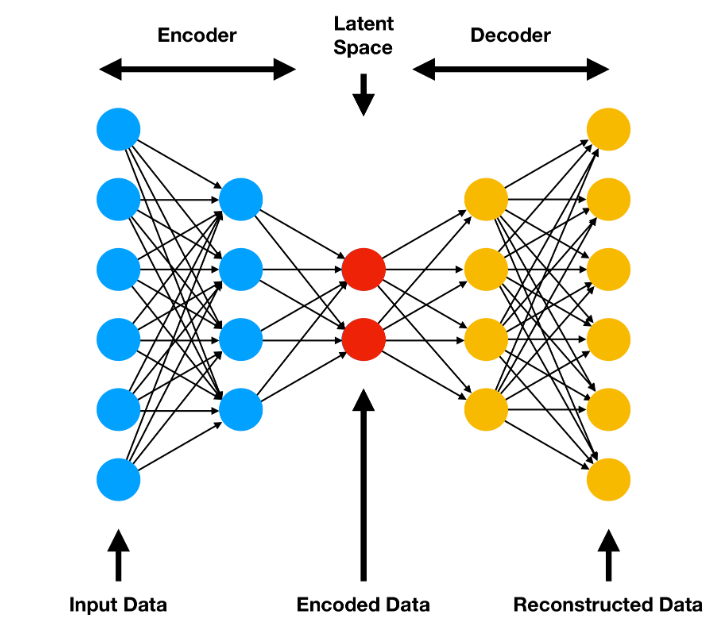
\includegraphics[width=\twoImgWidth]{images/autoencoder}%
    }%
    \hfill%
    \subfloat[\label{fig:sparseMatrix}]{%
      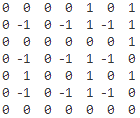
\includegraphics[width=\twoImgWidth]{images/sparse_matrix_game}%
    }%
    \captionadjust%
    \caption{\label{fig:autoencoderSparseMatrix}
    \protect\subref*{fig:autoencoder}: Example of an autoencoder network \cite{Img:autoencoder}.
    \protect\subref*{fig:sparseMatrix}: The 7x7 game state is getting more and more sparse over time.
    }%
\end{figure}

In our past work on Bomberman, we recognized the critical importance of state representation in optimizing the performance 
of our AI agents. Specifically, we focused on the transition from the original 17x17 grid, which encompassed the entire Bomberman field, 
to a reduced 7x7 grid. To accomplish this, we centered the agent's viewpoint in the 17x17 grid to capture the immediate surroundings. 
This reduction was not just a matter of simplification, it is especially important to prevent overfitting~\cite{Art:Overfitting}. When the agent network consistently 
receives the entire 17x17 field for learning, there's a high likelihood that the network will memorize training patterns and struggle with test data. 
The objective is to ensure that the agent learns the intelligent strategies of the rule-based agent to a certain extent, at the very least, mastering how 
to play the game effectively without necessarily striving for extreme efficiency. In doing so, we also took inspiration from humans who, like our AI, do not perceive 
the entire field but rather focus on a specific part while filtering out the rest.
Reducing the field to 7x7 retained key spatial relationships 
and relevant game features while simplifying the representation, thus allowing our AI agents to focus on essential information.
To determine if there is a difference in how the rule-based agent plays the game when the view box is reduced to 7x7, we had the following idea:
lets consider the following function: 
\begin{equation} \label{eq:1}
G_A(f,v) \rightarrow \{\text{up, down, left, right, bomb}\}
\end{equation}

that outputs the best possible action the agent could do. The field is described by $f$ and $v$ is the viewbox of the agent. We did many 
test rounds with the rulbased agent on an 17x17 field with \verb|--seed 1| for a comparable result. We had two scenarios
in one scenario the rulbased agent saw the whole 17x17 field e.g $G_a(f, 17\times17)$, on the other scenario the agent saw a
7x7 field e.g $G_a(f, 7\times7)$. Then we calculated the probability $p$ to find out how likely it is, that the actions in both scenarios are different in one step.
We simply counted the number of different actions and divided them by the maximum number of steps.
For the 7x7 field we had a probability of $p=0.054$ which was the best value for us compared to a 5x5 or 3x3 viewbox.\\

But, please note that initially, we interpreted this number $p$ quite differently. The probability distribution is not uniform. 
It turns out that the agent with a 7x7 viewbox makes more diverse actions as the game progresses compared to the agent with a 17x17 viewbox. 
This happens because towards the end of the game, there are fewer items or opponents within the 7x7 view, and the agent becomes uncertain about its actions. 
A better approach would be to determine the probability distribution function $p(X = k)$, where $k$ represents the number of steps in a game.
For example lets look at the probability at the beginning of the game $p(0 \geq X \leq 20) = 0$ and at the end of the game $p(310 \geq X \leq 330) = 0.47$
We had to come up with a solution to address this issue. Once the 7x7 field was empty of items or opponents, the agent switched to an exploration mode and randomly 
searched the surroundings for potential objectives.\\

However, the 7x7 field often contained sparse feature data see \autoref{fig:sparseMatrix}, with many cells remaining empty or irrelevant. 
To efficiently handle this challenge, we employed an encoder-decoder network see \autoref{fig:autoencoder}. This architecture allowed us 
to compress the sparse feature data effectively~\cite{Onl:autoencoder}. But before we delve into how the encoder-decoder network functions, we need to address how our 
features are generated within the \verb|state_to_features| function. First, we restrict the agent's field of view to 7x7. Then, we create a 7x7 map 
with the agent in the center, represented by the number 100. Here, 0 denotes open space, 1 represents crates, -1 signifies walls, 5 indicates coins, 15 represents 
opponents, and 25 stands for bombs. Another 7x7 map contains the hidden features, which are features that would otherwise overlap with those on the first map. 
These hidden features include whether all agents can ignite a bomb, represented as 0 or 1. A third map with hidden features describes the blast radius of a 
bomb along with its respective countdown. These three 7x7 maps, also known as channels, are then merged into a 
single 147-element array. Below is a code snippet:

\begin{lstlisting}[language=Python]
    ...

    def state_to_features(game_state: dict) -> np.array:
        field = game_state["field"]
        bombs = game_state["bombs"]
        explosion_map = game_state["explosion_map"]
        coins = game_state["coins"]
        agent = game_state["self"]
        others = game_state["others"]

        my_pos = make_field(agent[3])

        ...

        # non hidden features
        # make_field create a matrix from coordinate list
        channel1 = make_field(bombs) + make_field(others) + make_field(coins) 
                                     + field + my_pos

        # can agent put a bomb
        channel2 = extract_bom_is_possible_to_field(others) +  
                   extract_bom_is_possible_to_field(agent)

        channel3 = make_real_explosion_map(bombs, explosion_map)

        ...

        vf = make_viewbox(7,7, [channel1, channel2, channel3])
        return vf.flatten()

    ...
    
\end{lstlisting}

Next, we want to modify the \verb|state_to_features| function to further compress the data in the 149-element array while preserving as much information as possible. 
To achieve this, we'll utilize an encoder-decoder network see \autoref{fig:autoencoder}. This network has the same output dimension as the 
input dimension and aims to reconstruct the 
input data. However, in the dense layers, the features are reduced up to a certain point (encoded data layer). Then, in subsequent dense layers, the 
features are expanded back to the input dimension. If the network can effectively reconstruct the input data, we'll use it and extract the encoded data layer, 
which we will return in the \verb|state_to_features| function. We were able to compress the data from the 149-element array to a 72-element array. These data will 
now be used for our second network to train the rule-based agent. Details about both networks will be explained later 
in Model Architecture. Here's the modification of the \verb|state_to_features| function once again:

\begin{lstlisting}[language=Python]
    ...

    def state_to_features(game_state: dict) -> np.array:

        ...

        vf = make_viewbox(7,7, [channel1, channel2, channel3])
        compressed_features = encoder_decoder_network.encode(vf.flatten(), 72)
        return compressed_features

    ...

\end{lstlisting}

The encoder module was instrumental in feature learning, condensing the sparse data to capture essential features efficiently. 
Additionally, it reduced dimensionality, enhancing computational efficiency and reducing noise in the data. During decoding, the network could 
reconstruct the original 7x7 state representation from the compressed data, ensuring that no critical information was lost in the process.

\subsubsection*{Model Architecture}

\begin{figure}[H]
    \centering
    
    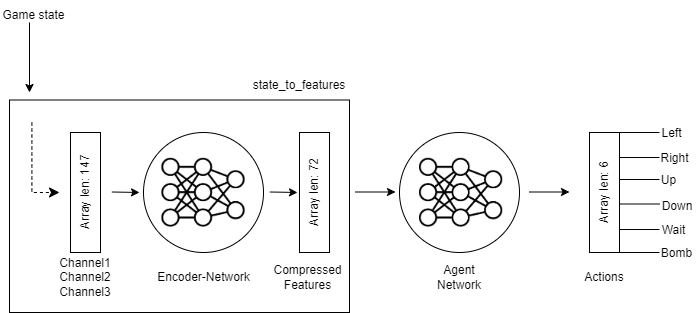
\includegraphics[width=\oneImgWidth]{images/network-arch}%
    
    \captionadjust%
    \caption{\label{fig:network-arch} Here is how our two models come into play.
    }%
\end{figure}

In total, we employ two neural networks see \autoref{fig:network-arch}. The encoder network is utilized within the \verb|state_to_features| function to compress the 
generated features, as they contain many repetitive entries, such as 0, 1, or -1. Through this compression, our aim is not only to reduce 
the data size but also to create patterns that make it easier to describe a state~\cite{Onl:autoencoder}. This is particularly significant for the second network. 
The second network is the agent network, which receives data from the \verb|state_to_features| function and endeavors to predict the best action.
Here are the characteristics of the two networks listed:

\begin{verbatim}
Encoder Network:
    Layers: 1 Inupt, 5 Hidden, 1 Output
    Neurons: 
        Input1: 147, Hidden1: 124, Hidden2: 102, Hidden3: 72,
        Hidden4: 102, Hidden5: 124, Output1: 147

Agent Network:
    Layers: 1 Inupt, 3 Hidden, 1 Output
        Neurons: 
            Input1: 72, Hidden1: 64, Hidden2: 32, Hidden3: 16, Output1: 6
\end{verbatim}

\subsubsection*{Loss function and optimizer}

We have two models: the encoder network for further feature compression and the agent network, which is tasked with 
learning how to play the game effectively. Additionally, the agent is initially meant to imitate the rule-based agent, which is 
achieved through classification. Later on, the agent will be further improved using deep Q-learning. For all these scenarios, we require 
different loss functions and optimizers with varying learning rates because there are more suitable optimizers and loss functions for specific cases.\\

For the encoder network, the ADAM optimizer with a learning rate of $0.001$ proved to be the most effective, and the chosen loss 
function was the MSE (Mean Squared Error) loss. During experimentation, we observed that the loss function did not converge to near 
zero with a learning rate of $>0.001$, and with a learning rate of $<0.001$, it converged towards zero, albeit very slowly. \\

For the agent network when mimic the rulbased agent, we used the ADAM optimizer with a learning rate of $0.0001$ and the Cross-Entropy loss function because
in classification, the goal is to assign probabilities to each class. Cross-entropy loss directly deals with probability 
distributions and can handle multi-class problems efficiently~\cite{Onl:crossentr}.\\

For the agent network during deep Q-learning, we used the ADAM optimizer with a learning rate of $0.0001$ and the Huber loss as the loss function.
It is designed to balance the benefits of mean squared error (MSE) and mean absolute error (MAE) loss functions.
But for any reason was the MSE loss better for the encoder network than the Huber loss.

\subsection{Other aproaches that we had}

At the beginning of the project, we had several other ideas about how to construct our AI agent. One alternative idea was to use Q-tables. 
For the coin collector agent, we considered the concept that it would only perceive one coin, specifically the one closest to it.
However, in the end, we discarded all of these ideas, and the following reasons explain why:

\subsubsection{Q-Tables}

Q-tables (Quality or Q-value tables) are used to approximate and store the expected cumulative rewards (Q-values) associated 
with different state-action pairs in a Markov Decision Process (MDP).
Rows represent states or state descriptions, columns represent possible actions that can be taken in those states.
Each cell in the table stores the expected cumulative reward, denoted as Q-value, for taking a specific action in a specific state.

The Q-value for a state-action pair $(s, a)$ represents the expected sum of rewards an agent can achieve by taking 
action $a$ in state $s$ and following a specific policy thereafter. The Q-value is typically updated iteratively as the 
agent explores and learns from its interactions with the environment.
Once the Q-table has converged or reached a sufficiently accurate representation of the optimal Q-values, 
the agent can select actions that maximize these Q-values

The equation for updating the Q-table in the context of Q-learning is as follows:
\begin{equation} \label{eq:1}
Q(s, a) = (1 - \alpha) \cdot Q(s, a) + \alpha \cdot [R(s, a) + \gamma \cdot \max_a Q(s', a)]
\end{equation}

In this equation:

\begin{itemize}

\item $Q(s, a)$ represents the Q-value for a specific state-action pair (s, a).
\item $\alpha$ (alpha) is the learning rate, determining the weight given to the new information when updating the Q-value. It's a value between 0 and 1.
\item $R(s, a)$ is the immediate reward received after taking action 'a' in state 's'.
\item $\gamma$ (gamma) is the discount factor, which controls the importance of future rewards. It's also a value between 0 and 1.
\item $Q(s', a)$ represents the Q-value of the next state 's' after taking action 'a', and \(a\) is the action that maximizes this Q-value.

\end{itemize}

The rason why we discarded this idea is that the bomberman environment has a large number of states, even when using a reduced state representation. 
Each cell on the game board can have multiple attributes (e.g., walls, crates, coins, enemies, bombs), resulting in an extensive state space. 
Creating a Q-table to store Q-values for every state-action pair in such a high-dimensional space would be impractical~\cite{Onl:qtabledis}.


\subsubsection{Coin-Collector Agent that sees only one coin}

Our coin collector agent was given the entire 17x17 field but only focused on the nearest coin, which was simply added to the \verb|game_state["field"]|. 
It received rewards only when collecting this specific coin. This approach worked very well for us, and the agent could consistently collect nearly 
all the coins later in the game. The advantage of this method is that it doesn't matter how many coins are on the field; the agent doesn't need to be 
retrained. However, for an agent tasked with more complex actions like defeating enemies, destroying crates, and collecting bombs, we couldn't 
pursue this idea. This is because we explored other concepts to enable the agent to perform various tasks effectively, and these concepts are described in this report.